\documentclass{article}
\usepackage{graphicx}
\usepackage{amsmath}
\usepackage{amssymb}
\usepackage{physics}
\usepackage{braket}

\title{Notes}
\date{}
\begin{document}
\maketitle
\section{Conjugate Gradient Method}
\subsection{Overview}
The conjugate gradient method (cgm) is an algorithm used to solve a linear system of the form
\begin{equation}
    Ax = b
\end{equation}
Where $A$ is a symmetric ($A^T=A$) positive definite ($x^TAx>0$) $n\times n$ matrix, $x,\ b$ vectors.
\\The algorithm is iterative, starting from a guess solution $x_0$ and taking a step towards the solution at each cycle.
\\The search directions are calculated from the residual term, defined as $r_i=b - Ax_i$. 
\\It is possible to prove that by choosing the step direction to be A-orthogonal to all the previous ones, the solution converges the fastest (i.e. the error term $\norm{e_i}=\norm{x_i-x}$ is minimized).
\subsection{Steepest descent}
A simpler algorithm is the steepest descent.
\\The idea is to take a step in the direction of the residual so that the quadratic form is minimized.
\begin{equation}
    x_{i+1} = x_i + \alpha_i r_i 
\end{equation}
\begin{equation}
    \alpha_i \text{ such that } \frac{d f(x_{i+1})}{d\alpha_i} = 0 \implies \alpha_i = \frac{r_i^T r_i}{r_i^T A r_i}
\end{equation}
This method is inefficient as $x_i$ often finds itself oscillating around the solution, since the search directions explore non-disjoint subspaces.
\subsection{The algorithm}
A better alternative is to set the search direction to be A-orthogonal to the error at the next iteration. If this is the case, it can be proven that the components of the error term are reduced to zero at each iteration, implying a convergence to the exact solution in $n$ steps.
\begin{equation}
    d^T_i Ae_{i+1} = 0 \implies \frac{d f(x_{i+1})}{d\alpha_i} = -r_{i+1}^T d_i = 0
\end{equation}
\begin{equation}
    \alpha_i = \frac{r_i^T d_i}{d_i^T A d_i}
\end{equation}
By definition, the residual is orthogonal to the previous search directions, we also have $r_i^T r_j=\gamma{ij}$. Since
\begin{equation}
    r_{i+1} = -A(e_{i+1}) = -A(e_i + \alpha_i d_i) = r_i - \alpha_i A d_i
\end{equation}
\subsubsection{Procedure}
The cgm algorithm can be summed up as follows:
\\Start with a guess solution $x_0$.
\\Let the first direction be the residual in $x_0$
\begin{equation}
    d_0 = r_0 = b-Ax_0
\end{equation}
Now, at each iteration, we can compute
\begin{align*}
    \alpha_i = \frac{r_i^T r_i}{d_i^T A d_i}  
    \\x_{i+1} = x_i + \alpha_i d_i
    \\r_{i+1} = r_i - \alpha_i A d_i
    \\\beta_{i+1} = \frac{r_{i+1}^T r_{i+1}}{r_i^T r_i}
    \\d_{i+1} = r_{i+1} + \beta_{i+1} d_i
\end{align*}

%Start with a guess solution $x_0$.
%\\Calculate the residual $r_0=b-Ax_0$.
%\\In terms of quadratic form, $r_0$ is the opposite of the gradient of $f(x)=x^TAx-b^Tx$, whose minimum is the solution of the linear system.

\subsection{Preconditioning}
The rate of convergance of cgm depends on the conditioning of the matrix $A$, defined as $\kappa(A)=\frac{\max{\lambda_i}}{\min{\lambda_i}}$, where $\lambda_i$ are the eigenvalues of the matrix.
\\The closer $\kappa(A)$ is to 1, the faster the convergence of the method.
\\Given a certain matrix $M$, symmetric, positive definite and easily invertible and such that $M^{-1}A$ has better conditioning than $A$, which is to say $M$ well approximates $A$, we can hope to solve the problem
\begin{equation}
    M^{-1}Ax = M^{-1}b 
\end{equation}
much faster than the original problem, where the two solutions will be the same.
\\The problem is that $M^{-1}A$ is not necessarily symmetric or positive definite.
\\The fact that $\exists E$ such that $M=EE^T$ and $E^{-1}AE^{-T}$ is symmetric and positive definite, we can solve the problem.
\begin{equation}
    E^{-1}AE^{-T}x = E^{-1}b
\end{equation}
By using some clever substitutions, we can go back to the original problem with the aid of the preconditioner, giving the following algorithm
\begin{align*}
    r_0 = b - A x_0 \\
    d_0 = M^{-1} r_0 \\
    \alpha_i = \frac{r_i^T M^{-1} r_i}{d_i^T A d_i} \\
    x_{i+1} = x_i + \alpha_i d_i \\
    r_{i+1} = r_i - \alpha_i A d_i \\
    \beta_{i+1} = \frac{r_{i+1}^T M^{-1} r_{i+1}}{r_i^T M^{-1} r_i} \\
    d_{i+1} = M^{-1} r_{i+1} + \beta_{i+1} d_i
\end{align*}

\section{Finding the smallest eigenvalue}
Finding the smallest/biggest eigenvalue-eigenvector pair of a matrix amounts to evaluating the unconstrained minimum/maximum of the Reyleigh quotient
\begin{equation}
    \lambda(x)=\frac{x^T Ax}{x^T x}
\end{equation}
Or, more generally
\begin{equation}
    Ax = B\omega x \implies \lambda(x)=\frac{x^T Ax}{x^T Bx}
\end{equation}
$\lambda$ is not a quadratic form, hence the cgm needs to be modified to use it.
\subsection{Useful multivariable relations}
Given $f(x)=x^T Ax$ and taking the derivative of $f$ in the direction of $v$
\begin{equation}
    f(x+hv) = (x+hv)^T A(x+hv) = f(x) + hv^T A x + hx^T A  v + o(h)
\end{equation}
\begin{equation}
    \dv{f}{v} = \lim_{h\to 0} \frac{f(x+hv)-f(x)}{h} = v^T Ax + x^T A v = v^T A x + v^T A^T x
\end{equation}
We can now evaluate the gradient of $f$ in x
\begin{equation}
    \nabla_x f(x) = \dv{f}{v} (x) = (A+A^T)x
\end{equation}
We can now take the gradient of the Rayleigh quotient
\begin{equation}
    \nabla \lambda(x) = \frac{(A+A^T)xx^T Bx - (B+B^T)x x^T Ax }{(x^T Bx)^2} 
\end{equation}
Using the fact that $A$ and $B$ are symemtric
\begin{equation}
\nabla \lambda(x)=2\frac{ Axx^T Bx - Bxx^T Ax}{(x^T Bx)^2}=2\frac{Ax-\lambda(x)Bx}{x^T Bx}
\end{equation}
\subsection{Non linear conjugate gradient}
Using a non quadratic form as function to be minimized, the things that will change will be
\begin{itemize}
\item The step size $\alpha_i$ will be different, we may now have multiple zeros regarding the orthogonality of the gradient and search direction.
\item The factor $\beta$ to compute conjugated directions no longer has equivalent forms.
\item The residual needs to be computed each time as $-\nabla f(x_i)$
\end{itemize}
Let's take a look at each problem and find a workaround.
\subsubsection{Step size}
We ought to find the step size for which $\lambda$ is minimized at each iteration. Being non linear (and non quadratic), an approximation must be done.
\\We can Taylor expand the function around $x_i$, in the direction $\alpha d_i$, and find the minimum of the polynomial.
\\Regarding the Rayleigh quotient, it amounts to finding the positive roots of the following polynomial:
\begin{gather*}
a \alpha_i^2 + b \alpha_i + c = 0 \\
a = (d_i^T A d_i) (x_i^T B d_i) - (x_i^T A d_i) (d_i^T B d_i) \\
b = (d_i^T A d_i) (x_i^T B x_i) - (x_i^T A x_i) (d_i^T B d_i) \\
c = (x_i^T A d_i) (x_i^T B x_i) - (x_i^T A x_i) (x_i^T B d_i)
\end{gather*}
Being the search direction always descending, we can simply select the positive root.
\subsubsection{Factor $\beta$}
The choice for $\beta$ is neither trivial nor unique, different formulations lead to distinct convergence properties and applicabilities.
\\Two possible choices are
\begin{equation}
\beta_{i+1}^{\text{FR}} = \frac{r_{i+1}^T r_{i+1}}{r_i^T r_i} 
\quad \text{or} \quad 
\beta_{i+1}^{\text{PR}} = \max \left\{ \frac{r_{i+1}^T (r_{i+1} - r_i)}{r_i^T r_i}, 0 \right\}
\end{equation}
The max operation will restart the method if $\beta$ is negative in the Polak Ribière, guaranteeing convergence.
\subsubsection{Algorithm}
The algorithm for minimizing the Rayleigh quotient can now be formulated as follows.
\\Choose an initial guess $x_0$.
\\Set the first search direction as the residual in $x_0$: $d_0 = r_0 = -g(x_0)$.
\\At each iteration, we can compute
\begin{align*}
    \alpha_i \text{ such that } f(x+\alpha_i d_i) \text{ minimized}
    \\x_{i+1} = x_i + \alpha_i d_i
    \\r_{i+1} = - g(x_{i+1})
    \\\beta_{i+1} \text{ from one of the possible choices}
    \\d_{i+1} = r_{i+1} + \beta_{i+1} d_i
\end{align*}
Since $\lambda(x)$ is not a quadratic form, the algorithm won't converge in $n$ steps, so that we will need to check for convergence at each iteration.
\subsubsection{Stopping}
As suggested in [painless conjugate gradient], a possible stopping criterion can be to check whether 
\begin{equation}
    \norm{g(x_i)} < \epsilon \norm{g(x_0)}
\end{equation}

\section{Finite Differences}
We can employ discretization methods such as finite differences to approximate the solution of a differential equation.
\subsection{Second order ODEs}
The taylor expansion of a function $\psi(x\pm h)$ around a point $x$ is given by
\begin{equation}
    \psi(x\pm h) = \psi(x) \pm h \psi'(x) + \frac{h^2}{2!} \psi''(x) + \ldots
\end{equation}
\subsubsection{First and second derivative}
By subtracting $\psi(x+h)$ and $\psi(x-h)$, we get an approximation for the first derivative
\begin{equation}
    \label{eq:finite_diff_first_dv}
    \psi'(x) \approx \frac{\psi(x+h) - \psi(x-h)}{2h}
\end{equation}
By adding them, we can get an approximation for the second derivative
\begin{equation}
    \psi''(x) \approx \frac{\psi(x+h) - 2\psi(x) + \psi(x-h)}{h^2} \label{eq:finite_diff_2nd}
\end{equation}
\subsection{Discretization}
Given an eigenvalue boundary problem, formulated as
\begin{align}
    \psi''(x)  = f(x, \psi, \psi', E) \ \ \forall x \in [a, b] \label{eq:bvp_eigenvalue}
\end{align}
We can build a lattice of $n$ points
\begin{equation} 
    X = \{x_i = a + ih \ \forall i = 0, \ldots, n-1\}
\end{equation}
Writing $\psi(x_i) = \psi_i$, and the equation $\psi''_i = f(x_i, \psi_i, \psi'_i, E)$ $\forall i$ we get a linear system of the form
\begin{equation}
    A \underline{\psi} = E\underline{\psi}
\end{equation}
Finding the eigenvalues and eigenvectors of $A$ amounts to finding the solutions $\psi$ and the corrisponding eigenvalues $E$ of the eigenvalue problem \ref{eq:bvp_eigenvalue}.
\subsection{1D Harmonic oscillator}
In quantum mechanics, one often finds necessary to solve the reduced Schrödinger equation
\begin{equation}
    \hat H \psi = (\hat T + \hat V)\psi =E\psi 
\end{equation}
Where $\hat H$ is the Hamiltonian, a differential operator, and $E$ the energy associated to a state $\psi$.
\\A simple but rather useful example is the harmonic oscillator, where the potential is given by
\begin{equation}
    V(x) = \frac{1}{2}m\omega^2(x-x_0)^2
\end{equation}
\subsubsection{Harmonic oscillator and equilibrium}
The power of the harmonic oscillator comes from the fact that a system at equilibrium will roughly have its particles in the minium of the potential energy.
\\From a single particle point of view, we can say that the potential to which it's subjected is a function of its position $x$, which at equilibrium can be expanded as
\begin{equation}
    V(x) = V(x_0) + \dv{V}{x}\bigg|_{x_0}(x-x_0)+ \frac 1 2 \dv[2]{V}{x}\bigg|_{x_0}(x-x_0)^2
\end{equation}
Since the first derivative is zero at equilibrium, and the potential additive constant can be ignored, we can write
\begin{equation}
    V(x) = \frac{1}{2}m\omega^2(x-x_0)^2
\end{equation}
Where 
\begin{equation}
    m\omega^2 = \dv[2]{V}{x}\bigg|_{x_0}
\end{equation}

\subsection{Matrix solution}
Given the Hamiltonian
\begin{equation}
    \hat H = \frac{-\hbar^2}{2m}\dv[2]{}{x}+\frac 1 2 m \omega^2 x^2
\end{equation}
We can combine \ref{eq:bvp_eigenvalue} and \ref{eq:finite_diff_2nd}, using a step size $h$ to get
\begin{equation}
    \frac{(\frac C 2 m\omega^2 x_i^2 h ^2 - 2)\psi_j + \psi_{j-1} + \psi_{j+1}}{h ^2 C} = E\psi_j \label{eq:finite_diff_ho}
\end{equation}
Where $C = {-2m}/{\hbar^2}$.
\\The left hand side of \ref{eq:finite_diff_ho} gives the entries of matrix A, for which the smallest eigenvalue can be found by minimizing the Rayleigh quotient with the non linear cgm.
\subsubsection{Harmonic oscillator applied to nuclei}
A numerical solution to the harmonic oscillator is now given for the applied case of a nucleon in the nucleus.
\\The value of $\omega$ can be calculated from the empirical density of nuclei, which can be written as a function of $\sqrt{\braket{r^2}}$, analytically known in the case of an harmonic oscillator.
\begin{equation}
    \hbar \omega = \frac{41}{A^{1/3}} \text{MeV}
\end{equation}
\\This may seem tautological but the aim is to verify the validity of the numerical solution while seeing the method in action for a real case.
\\The mass of the particle is assumed to be 939 MeV.
\\A calculation was performed on a grid of 1000 points, in an interval $[-a, a]$ such that $a=10$ fm.
\\The resulting wavefunction is shown in figure \ref{fig:1D_ho}.
\\Assuming a mass number of $A=16$, the eigenvalue (energy) associated to the graound state is 8.143 MeV.
\\Since the computation was done in one dimension, a factor of 3 is needed to compare it to a real nucleus.
\\Assuming the nucleon to be bound through a potential well of $\approx$ 40 MeV, the separation energy will be $\approx$ 40 - 8.143 $\cdot$ 3 = 15.571 MeV.
\begin{figure}[!htb]
\centering
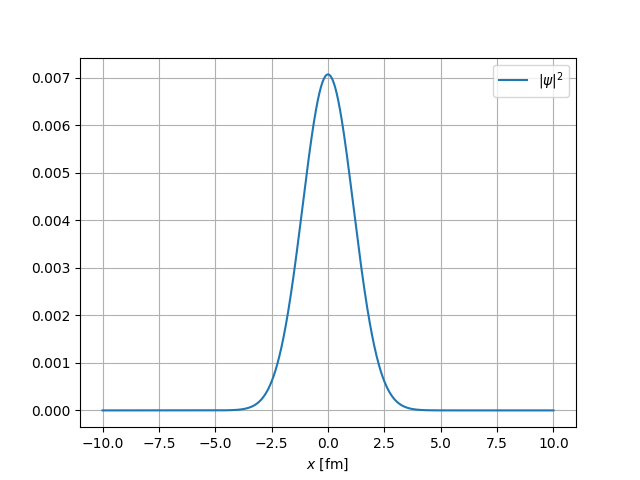
\includegraphics[width=0.8\textwidth]{figures/1D_ho.png}
\caption{\label{fig:1D_ho} Ground state wavefunction of the harmonic oscillator. The solution starts roughly vanishes for $|x|>3$ fm, as expected for a nucleus of this size.}
\end{figure}
\subsection{Second order PDEs}
The method of finite differences can be extended to second order PDEs.
\\For the moment, we will consider only a 2 dimensional problem, without losing generality.
\\Given the boundary eigenvalue problem
\begin{equation}
\pdv[2]{\psi}{x}+\pdv[2]{\psi}{y} = f(\psi, \pdv{\psi}{x}, \pdv{\psi}{y}, x, y, E)
\end{equation}
\\We can build a lattice of $N_x, N_y$ points as follows
\begin{equation}
    X = \{x_i = a_x + ih_x \ \forall i = 0, \ldots, N_x-1\}, \  Y = \{y_j = a_y + jh_y \ \forall j = 0, \ldots, N_y-1\}
\end{equation}
By applying the finite differences method on $x$ we get
\begin{equation}
    \pdv[2]{\psi_i}{y} + \frac{\psi_{i+1}(y) - 2\psi_i(y) + \psi_{i-1}(y)}{h_x^2} = f(\psi_i(y), \fdv{\psi_i}{x}, \pdv{\psi_i}{y}, x_i, y, E)
\end{equation}
Where the $\delta$ denotes the first partial derivative in the finite differences approximation.
\\We can now apply again the finite differences approximation to the $y$ coordinate, which yields
\begin{equation}
    \frac{\psi_{i, j+1}+\psi_{i, j-1}-2\psi_{i, j}}{h_y^2} + \frac{\psi_{i+1, j}+\psi_{i-1, j}-2\psi_{i,j}}{h_x^2} = f(\psi_{i, j}, x_i, y_j, \fdv{\psi_{ij}}{x}, \fdv{\psi_{ij}}{y}, E)\label{eq:finite_diff_2nd_pde}
\end{equation}
Rearranging the terms, it's possible to obtain the following system of equations:
\begin{equation}
    \sum_{i'j'}A_{i,j,i',j'}\psi_{i'j'} = E\psi_{i,j}\label{eq:hypermatrix_2d}
\end{equation}
Where $A_{i,j,i',j'}$ is a hypermatrix of size $N_x \times N_y \times N_x \times N_y$.
\\The next task will be to find a way to express $\ref{eq:hypermatrix_2d}$ as a linear system of equations, by finding a choice of index that encapsulates the relation for all pairs $(i, j)$, with the constraint that the resulting matrix is symmetric.
\\Formally
\begin{equation}
    F:(i,j)\mapsto \gamma \text{ such that }\alpha = F(i, j),\ \beta = F(i',j')\implies\ A_{\alpha\beta} = A_{\beta\alpha}
\end{equation}
This is guaranteed if the factors $A_{i,j,i',j'}$ are symmetric under the exchange  $i \leftrightarrow i'$ and $j \leftrightarrow j'$ and the map $F$ is bijective.
\begin{equation}
    A_{F(i,j),F(i',j')} = A_{i,j,i',j'} = A_{i', j', i, j} = A_{F(i',j'),F(i,j)}
\end{equation}
\subsubsection{Indeces parametrization}
A possible map $(i, j) \mapsto \gamma$ is
\begin{equation}
F(i, j) = \gamma = i + N_x j \label{eq:indeces_parametrization}
    \end{equation}
Using this map, the entries of $\psi_\mu$ will be organized as 
\begin{equation}
\psi = (\psi_{(0, 0)}, \psi_{(1, 0)}, \ldots, \psi_{(N_x-1, 0)}, \psi_{(0, 1)}, \ldots, \psi_{(N_x-1, N_y-1)})
\end{equation}
And the problem will be reduced to 
\begin{equation}
\sum_{\beta=0}^{N_x N_y}A_{\alpha\beta}\psi_{\beta} = E\psi_\alpha
\end{equation}
\subsubsection{3D case}
The 3D case follows trivially by performing discretization on the z-axis, adding a new index $k$ and using the map $F(i, j, k) = i + N_x (j + N_y k)$.

\subsubsection{Boundary conditions}
For a short range potential, we can expect bound solutions to decay rapidly near the boundaries, prompting for Dirichlet boundary conditions.
\\In a simple 1D case, where the domain is $[a, b]$, $\psi_0 = \psi(a)$, $\psi_{N-1} = \psi(b)$, the approximation for the derivatives asks for $\psi_{-1}$ and $\psi_N$.
\\Since we are not contemplating these points in the domain, we can simply set them to zero, which formally corresponds to solving
\begin{equation}
    \begin{pmatrix}
        0 & 0 & 0 
        \\0 & A & 0
        \\0 & 0 & 0
    \end{pmatrix}
    \begin{pmatrix}
        0\\\mathbf{\psi}\\0
    \end{pmatrix}
    = E 
    \begin{pmatrix}
        0\\\mathbf{\psi}\\0
    \end{pmatrix}
\end{equation}
This implies that the solution $\psi$ satisfies the boundary conditions for 
\begin{equation}
    \psi(a-h)=0 \text{ and } \psi(b+h)=0.
\end{equation}
\\Working with a sufficiently fine mesh, this slight deviation is physically negligible, since $h \approx 0$. Nonetheless, it's possible to satisfy the exact BC by working in the domain $[a+h, b-h]$. 

\subsection{Woods Saxon}
Now that the machinery for solving 3D eigenvalue problems is in place, we can apply to the Woods-Saxon potential.
\\The Woods-Saxon potential is a phenomenological one, it comes from the distribution of electric charge in a nucleus, which we can gather from electron scattering experiments.
\\The potential is assumed to have the same functional form, but with consants which are empirically determined as to fit the experimental data.
\\The potential is given by
\begin{equation}
    V_{\text{WS}}(r) = \frac{-V_0}{1+e^{\frac{r-R}{a}}}
\end{equation}
Where the usual parametrization is
\begin{gather}
    R=r_0A^{1/3} =1.27A^{1/3} \text{ fm} \\
    a = 0.67 \text{ fm}\\
    V_0 = \bigg(51\pm33\frac{N-Z}{A}\bigg) \text{ MeV}
\end{gather}
Solving the associated Hamiltonian on a lattice of $N_x=N_y=N_z=100$ points, in an interval of [-10, 10] fm for all three axes, we get a ground state energy of $-31.103 \text{ MeV}$ and the wavefunction in figure \ref{fig:ws_gs}.
\begin{figure}
    \centering
    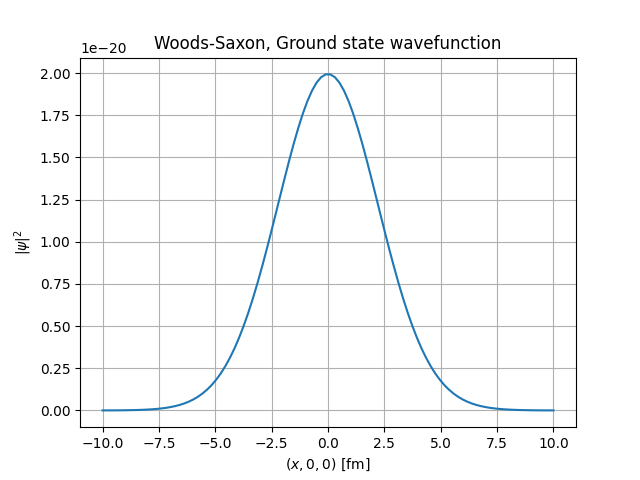
\includegraphics[width=0.8\textwidth]{figures/ws_gs.png}
    \caption{\label{fig:ws_gs} Ground state wavefunction of the Woods-Saxon potential. }
\end{figure}

\subsection{Spin}
In the case of this work, dealing with non relativisitic quantum mechanics, we treat spin as an additional degree of freedom of our single particle system.
\\Recalling the commutators that define the spin operator in 3 dimensions:
\begin{equation}
    [S_i, S_j] = i\hbar \epsilon_{ijk} S_k
\end{equation}
Where $\epsilon_{ijk}$ is the Levi-Civita symbol.
\\Spin comes into action by means of Spin Orbit interaction through the operator $\hat {\mathbf L }\cdot \hat{\mathbf S}$.
\\$\hat{\mathbf{L}}$ acts on the Hilbert space of position by $\hat{\mathbf L} = (\mathbf r \times \mathbf p )= -i\hbar (\mathbf r \times \nabla)$.
\\While $\hat{\mathbf S}$ acts on the Hilbert space of spin, a representation of $\text{SU}(2)$ where the basis vectors are its projection on the $z$ axis.
\\We can then rewrite by the pauli matrices $\hat{\mathbf S} = i\frac \hbar 2 \boldsymbol {\sigma}$, where 
\begin{equation}
    \boldsymbol{\sigma} = (\sigma_x, \sigma_y, \sigma_z) = \bigg( \begin{pmatrix} 0 & 1 \\ 1 & 0 \end{pmatrix}, \begin{pmatrix} 0 & -i \\ i & 0 \end{pmatrix},\ \begin{pmatrix} 1 & 0 \\ 0 & -1 \end{pmatrix} \bigg)
\end{equation}
\subsubsection{Spin and finite differences}
Working in 3D, together with spin, the lattice on which we want to solve our eigenvalue problem is given by sets of points $\mathcal{X}, \mathcal{Y}, \mathcal{Z}$ as done previously, while the spin, discrete by nature, can be represented by 
\begin{equation}
    \mathcal{S} = \{ -\hbar /2, \hbar / 2\}
\end{equation}
Since we're adding a "fourth" dimension to the problem, the transformations that maps all the different indeces to a single one will be
\begin{equation}
    F(i, j, k, s) = s + 2 (i+N_x(j+N_y k))
\end{equation}
Where 2 comes from the size of the spin representation.
\subsection{Parametrization and discretization of the spin orbit interaction}
In the case of the Woods Saxon potential, the spin orbit is phenomenologically parametrized as
\begin{equation}
    \hat {H}_\text{SO} = v_{\text{LS}}(\mathbf{r})\mathbf{L}\cdot \mathbf{S}
\end{equation}
Where 
\begin{equation}
    v_{\text{LS}}(\mathbf{r}) = v_{\text{LS}}^{(0)}\bigg(\frac{r_0}{\hbar}\bigg)^2\frac 1 r \bigg[\dv{r}\frac 1 {1+ e^{\frac{r-R}{a}}}\bigg]
\end{equation}
We can develop the product 
\begin{equation}
    \mathbf{L}\cdot \mathbf{S} = -i\frac {\hbar^2} 2 \bigg(\sigma_x \bigg(y\pdv{z} - z\pdv{y}\bigg) + \sigma_y \bigg(z\pdv{x} - x\pdv{z}\bigg) + \sigma_z \bigg(x\pdv{y} - y\pdv{x}\bigg)\bigg)
\end{equation}
Using finite differences, thanks to the approximation in equation \ref{eq:finite_diff_first_dv}, we are able to write the first partial derivatives in terms of $\psi$
\begin{align*}
    \pdv{\psi}{x} = \frac {\psi_{i+1, j, k} - \psi_{i-1, j, k}}{2h_x}
    ;&\ \pdv{\psi}{y} = \frac {\psi_{i, j+1, k} - \psi_{i, j-1, k}}{2h_y}
    ;&\ \pdv{\psi}{z} = \frac {\psi_{i, j, k+1} - \psi_{i, j, k-1}}{2h_z}
\end{align*}
It's obious that the matrix elements describing the spin orbit interaction will be off-diagonal, since they are non local.
\\The discretized $\hat H$, a matrix $2N_x N_y N_z\times 2N_x N_y N_z$ will then be the sum $T + V + H_{\text{SO}}$ of the kinetic energy, the potential energy and the spin orbit interaction. 


%\section{The Hartree-Fock method}
A many body system, like the nucleus, is made of indistinguishible particles from the standpoint of quantum mechanics.
\\Suppose to have a nucleus, with $A$ nucleons, where the mass difference between neutrons and protons is neglected.
\\The state of the system will be described by a wavefunction $\Psi(\mathbf{r_1}, \ldots, \mathbf{r_A})$.
\\The HF approximation states that the wavefunction can be approximated as a product of single particle states:
\begin{equation}
    \Psi(\mathbf{r_1}, \ldots, \mathbf{r_A}) = \prod_{i=1}^A \phi_i(\mathbf{r_i})
\end{equation}
Since we are dealing with fermions, the correct state must be antisymmetric with respect to a particle exchange, forcing the use of a slater determinant:
\begin{equation}
    \Psi(\mathbf{r_1}, \ldots, \mathbf{r_A}) = \frac{1}{\sqrt{A!}}\det
    \begin{pmatrix}
        \phi_1(\mathbf{r_1}) & \ldots & \phi_A(\mathbf{r_A}) \\
        \ldots & \ddots & \ldots \\
        \phi_1(\mathbf{r_A}) & \ldots & \phi_A(\mathbf{r_1})
    \end{pmatrix}
    =\sum_{p} (-1)^p \phi_{p(1)}(\mathbf{r_1}) \ldots \phi_{p(A)}(\mathbf{r_A})
\end{equation}
Where the sum is performed over all possible permutations of the particles.
\\Using the variational principle, we can determine the ground state by minimizing the energy functional
\begin{equation}
    \label{eq:energy_functional}
    E[\Psi] = \bra{\Psi} \hat{H} \ket{\Psi}
\end{equation}
With the constraint that the single particle states be orthogonal to each other.
\begin{equation}
    \delta E = \delta(\bra{\Psi} \hat{H} \ket{\Psi} - \sum_A \varepsilon_i\braket{\phi_i | \phi_i} ) = 0
\end{equation}
This variation, along with the constraint, gives rise to a single particle Schrodinger-like equation:
\begin{equation}
-\frac{\hbar^2}{2m} \nabla_i^2 \phi_i(\mathbf{r}) + \sum_{j=1}^A \int d^3 r' \ \phi_j^*(\mathbf{r}') v(\mathbf{r}, \mathbf{r}') \phi_j(\mathbf{r}') \phi_i(\mathbf{r}) - \sum_{j=1}^A \int d^3 r' \, \phi_j^*(\mathbf{r}') v(\mathbf{r}, \mathbf{r}') \phi_j(\mathbf{r}) \phi_i(\mathbf{r}') = \varepsilon_i \phi_i(\mathbf{r}).
\end{equation}
One can choose a proper potential $v(\mathbf{r_1}, \mathbf{r_2})$, a trial set of wavefunctions, and solve for $(\phi_i, \varepsilon_i)$.
\\Since the equation changes for the new solutions, one can use an iterative procedure to solve the self consistent problem.


\end{document}

